\chapter{Konzeption} % Das würde eigentlich 'Konzeption' heißen aber Tichy wirkt stark in mir

hier kurz beschreiben, was so grob abgeht, also was wir so machen wollen und was für netze wir vergleichen wollen,
um das beste zu finden

\section{Architektur}

Im Folgenden werden die untersuchten Architekturen genauer beschrieben und ebenfalls begründet, 
warum die jeweiligen architektonischen Entscheidungen getroffen wurden. \\
In \autoref{sec:state-of-the-art-roads} wurde ausführlich der Stand der Technik und Wissenschaft 
im Bereich der Straßenerkennung und -extraktion mittels Computer-Vision-Modellen beschrieben. 
Aufgrund der Ähnlichkeit der Problemdomäne lässt sich vermuten, dass ähnliche Verfahren wie 
zum Erkennen von Straßen auch für das Erkennen von Fahrradwegen nützlich sein könnten. 
Die Problemdomänen sind ähnlich, da Fahrradwege auch Straßen sind und eben jene Eigenschaften, 
wie große Klassenimbalance zwischen Fahrradweg und Hintergrund, Beschattung durch andere Objekte,
Verdeckung durch z.B. Bäume und ähnliche Annotationsfehler   
teilen. Schwierigkeit hier wird sein, Fahrradwege von Straßen zu unterscheiden. \\
Die Radwege sollen, wie Straßen auch, mittels Image-Semantic-Segmentation von einem Computer-Vision-Modell 
markiert werden. Andere Klassifizierungsarten, wie die in \autoref{sec:aufgabenkategorien} beschriebene 
Objektdetektion würde zu grobe Bounding-Boxes um schräg verlaufende Radwege legen, sodass im Prinzip 
eine Straße markiert werden würde, die zwar ein Radweg hat, aber nicht klar wäre, wo dieser verläuft, 
bzw. ob ein Radweg in beide Richtungen existiert. Aus demselben Grund ergibt eine reine Klassifikation, 
ob ein Bild ein Radweg enthält oder nicht ebenfalls keinen Sinn. 
Auf der anderen Seite würde Instanz-Segmentierung keine weiteren relevanten Informationen hinzufügen, 
wonach semantische Segmentierung völlig ausreicht, um das Problem zu lösen. \\
Wie bereits in \autoref{sec:state-of-the-art-roads} dargelegt sind alle relevanten Modelle zur 
Straßenerkennung basierend auf der U-Net-Archtiektur (vgl. \ref{sec:architekturkomponenten:unet}).
Folglich sollen die hier betrachteten Modelle ebenfalls als angepasste U-Nets entworfen werden. 
Insbesondere ermöglicht dies auch die Modelle zur Fahrradwegerkennung auf den verschiedenen 
in \autoref{sec:roads-data} vorgestellten Datensätzen zur Straßenerkennung vorzutrainieren, 
was zu allgemein besseren Ergebnissen führen kann (s. \autoref{sec:transfer-learning}). 
Außerdem können so die erzielten Ergebnisse vom Pre-Training mit den öffentlichen Benchmarks verglichen werden,
um deren Ergebnisse zu validieren und früh Fehler in den eigenen Entscheidungen und Implementationen zu entdecken.

Zunächst soll so ein nur leicht modifiziertes U-Net, welches im Folgenden \textit{Bike-U-Net} 
genannt wird, entworfen werden, welches als Baseline- und Vergleichs-Netz dienen soll.
Dann soll eine zweite Klasse an U-Nets beschrieben werden, die verschiedene vortrainierte \acp{CNN} (s. \autoref{sec:pretrained-backbones}) 
als Backbones für ein U-Net verwendet, da \autoref{sec:state-of-the-art-roads} gezeigt hat, 
dass im Falle der Straßendetektion die Performanz eines Netzes stark verbessert werden konnte, 
indem auf Techniken und Methoden von Modellen aus anderen Teilgebieten der Computer-Vision 
zurückgegriffen wurde. Die einfachste Ausprägung hiervon ist das Dense-U-Net-121, 
welches einfach ein DenseNet121 als Backbone verwendet und somit von dessen Pre-Training und Architektur
profitieren konnte und damit 2-5\% bessere Resultate in der Basline-Bewertung und bis zu 19\% 
bessere Ergebnisse in der optimierten Version erzielen konnte, als ein herkömmliches U-Net. 
Gegebenenfalls ist das auch für die Radwegerkennung möglich. Dazu sollen mehrere Backbones untersucht werden. 

\subsection{Bike-U-Net}

\begin{figure}
	\centering
	\includegraphics[width=1.\textwidth]{Bilder/own-unet-2mil.pdf} 
	\caption{CAPTION 1,946 Mio Param.}
	\label{fig:own-unet-2mil}
\end{figure} 


\subsection{Backbone-U-Nets}


WARUM ELU? 
Kein vanishing gradient, recht schnell zu berechnen, kein dying neuron problem (insb. elevant bei CNN (u-net paper quoten)), blow up von aktivierung wird gedämpft durch batch norm. 


\section{Algorithmus zur Reduktion eines Materialflussgraphen} \label{sec:reduction}

Beim Reduzieren der Submodellgraphen ist es wichtig die Wert-Information der reduzierten Knoten nicht zu verlieren. Hierzu werden zuerst die Werte der Knoten aus $R$ zu dem jeweils topologisch-sortiert nächsten Knoten $f \in F$ propagiert, der von einem $r \in R$ erreichbar ist. \\
Folglich wird zunächst $G$ topologisch sortiert. Dann wird über diese Sortierung iteriert. Ist der derzeitige Knoten in $R$, so wird sein Wert auf den Wert des per Definition einen Nachfolgerknotens addiert. Ist der derzeitige Knoten in $F$, wird nichts unternommen. Die topologische Sortierung garantiert, dass alle Vorgängerknoten eines Knoten in $R$ ihren Wert propagiert haben, bevor er selbst seinen Wert propagiert. \autoref{lst:prop} stellt den eben beschriebenen Algorithmus dar.

\begin{algorithm}
	\caption{Algorithmus zum Propagieren und Akkumulieren von Knotenwerten.}\label{lst:prop}
	\begin{algorithmic}[1]
		\Procedure{Reduce}{$G = (V,E)$} \Comment{$\forall v \in V: value(v) = weight(type(v))$}
			\State $sortedNodes \gets topoSort(G)$
			\For{$v \in sortedNodes$}\Comment{iteration in topological order}
				\If{$v \in R$} 
					\State $succ \gets successor(v)$ \Comment{$d^+_G(v) = 1$}
					\State $value(succ) \gets value(succ) + value(v)$
				\EndIf
			\EndFor
		\EndProcedure
	\end{algorithmic}
\end{algorithm}

Nun da alle Knoten die neuen kumulierten Werte haben, lassen sich die reduzierbaren Knoten $r \in R$ entfernen. 

\mathchardef\mhyphen="2D

\begin{algorithm}
	\caption{Algorithmus zum Kopieren nötiger Kanten von reduzierten Knoten.}\label{lst:reduce}
	\begin{algorithmic}[1]
		\Procedure{Reduce}{$G = (V,E), C = (F, E_F)$} \Comment{$E_F = \emptyset$}
			\State $sortedNodes \gets topoSort(G)$
			\For{$v \in sortedNodes$}\Comment{iteration in topological order}
				\If{$v \in F$} 
					\For{$succ \in successors(v)$}\Comment{$d^+_G(v) \neq 1$}
						\If{$succ \in F$}
							\State $E_F \gets E_F \cup \{(v, succ)\}$ \Comment{copy $fork \rightarrow fork$}
						\EndIf
					\EndFor
				\Else \Comment{$v \in R$}
					\State $succ \gets successor(v)$ \Comment{$d^+_G(v) = 1$}
					\For{$pred \in predecessors(v)$}
						\If{$pred \in F \land succ \in R$}
							\State $E \gets E \cup \{(pred, succ)\}$\Comment{connect $fork \rightarrow non \mhyphen fork$}
						\ElsIf {$pred \in F \land succ \in F$}
							\State $E_F \gets E_F \cup \{(pred, succ)\}$ \Comment{copy $fork \rightarrow fork$}
						\EndIf
					\EndFor
				\EndIf
			\EndFor\label{euclidendwhile}
		\EndProcedure
	\end{algorithmic}
\end{algorithm}

\pagebreak % manueller seitenumbruch

\section{Gänzliche Einsparung gemeinsamer Teilgraphen} \label{sec:skip_entirely}

\begin{wrapfigure}{l}{0.35\textwidth}
	\centering
	\vspace{-30pt} % Manchmal möchte man den oberen Abstand selbst anpassen
	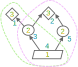
\includegraphics[width=0.30\textwidth]{Bilder/problem_illustration.pdf}
	\vspace{-10pt}
	% Das folgende ist ein Trick, um "Abbilgung x.y" in eine
	% eigene Zeile zu packen. Der Text zwischen [ und ] steht
	% im Abbildungsverzeichnis. Der Text darunter wird
	% tatsächlich angezeigt.
	\caption[Minimalbeispiel zur Teilgraph-Überspringungs-Problematik. Legende wie in \autoref{fig:trans_closures}.]{\unskip}
	Minimalbeispiel zur Teilgraph-Überspringungsproblematik. Legende wie in Abb. \ref{fig:trans_closures}.
	\label{fig:prob_illu}
\end{wrapfigure}

Leider lassen sich bei dem Vergleich zweier Submodelle gemeinsame Teilgraphen nicht gänzlich einsparen, indem der Similarity-Wert über Forks hinaus propagiert wird, um so jedem Knoten im Graph die Summe aller Knotenwerte unter ihm zuzuordnen, da ein gemeinsamer Teilgraph über mehrere Forks betreten werden kann (z.B. der Teilgraph der Schnittmenge von grün und lila in \autoref{fig:trans_closures} kann über Knoten 6 und 5 betreten werden) und nur der maximale Teilgraph gezählt werden darf - ansonsten würde es zu einer doppelten Wertung eines oder mehrerer Knoten kommen. Auch ist die Maximalität  des gemeinsamen Teilgraphen nur mit erheblichen Rechenaufwand, der dem Prinzip des Auslassens entgegensteht, zu überprüfen. Der Graph aus \autoref{fig:prob_illu} ist zur Veranschaulichung geeignet: Es ist schwierig Knoten 4 mit Wert 1 genau einmal zu zählen. Wird Knoten 3 betreten und der restliche Teilgraph (Knoten 4) übersprungen, so wird der Wert 3 zur Similarity addiert.
